\documentclass{beamer}
\usepackage{listings}
\lstset{
%language=C,
frame=single, 
breaklines=true,
columns=fullflexible
}
\usepackage{subcaption}
\usepackage{url}
\usepackage{tikz}
\usepackage{tkz-euclide} % loads  TikZ and tkz-base
%\usetkzobj{all}
\usetikzlibrary{calc,math}
\usepackage{float}
\newcommand\norm[1]{\left\lVert#1\right\rVert}
\providecommand{\pr}[1]{\ensuremath{\Pr\left(#1\right)}}
\providecommand{\sbrak}[1]{\ensuremath{{}\left[#1\right]}}
\providecommand{\brak}[1]{\ensuremath{\left(#1\right)}}
\providecommand{\fourier}{\overset{\mathcal{F}}{ \rightleftharpoons}}
\providecommand{\ztrans}{\overset{\mathcal{Z}}{ \rightleftharpoons}}
\providecommand{\abs}[1]{\left\vert#1\right\vert}
\renewcommand{\vec}[1]{\mathbf{#1}}
\usepackage[export]{adjustbox}
\usepackage[utf8]{inputenc}
\usepackage{amsmath}
\usetheme{Boadilla}

\title{GATE EC 2001 - Q.16}
\author{Tanmay Goyal - AI20BTECH11021}

\date{}

\begin{document}

\begin{frame}
\titlepage
\end{frame}
\begin{frame}
\frametitle{Question}
\begin{flushleft} 
\begin{columns}
\begin{column}{0.5\textwidth}
\begin{figure}[!ht]
\centering
 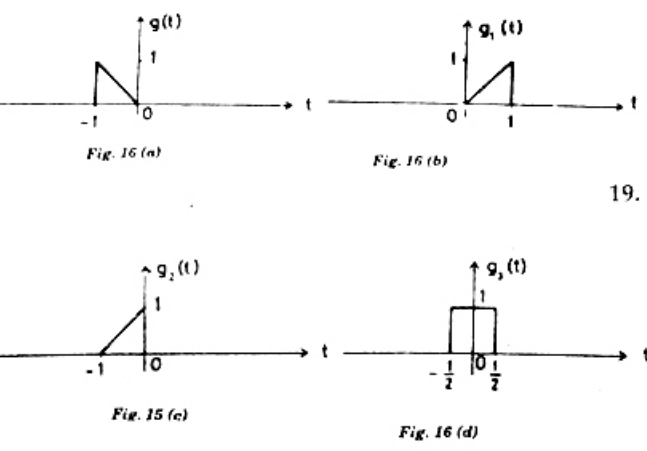
\includegraphics[width=\columnwidth]{Question.png}
\end{figure}
\end{column}
\begin{column}{0.5\textwidth}
The Fourier Transform $G(f)$ of the signal $g(t)$ is given by 
\begin{align}
    G(f) = \frac{1}{4\pi^2 f^2}(e^{2\pi jf} - 2\pi jf e^{2\pi jf} -1)
\end{align}
Using this information, find the Fourier Transforms of the signals $g_1(t)$, $g_2(t)$ and $g_3(t)$.
\end{column}
\end{columns}

 
\end{flushleft}
\end{frame}

\begin{frame}[fragile]
\frametitle{Result of Time Shifting on Fourier Transform}

\begin{flushleft}
\begin{lemma}
If 
\begin{align}
    g(t) \fourier G(f)
\end{align}
then,
\begin{align}
    g(t \pm t_0) \fourier G(f)e^{\pm 2\pi j f t_0}
\end{align}
\label{shift}
\end{lemma} 
\begin{proof}
We know, 
\begin{align}
    G(f) = \int_{-\infty}^\infty g(t) e^{-2\pi j ft} \,dt
\end{align}
\end{proof}
\end{flushleft}
\end{frame}


\begin{frame}[fragile]
\frametitle{Proof continued}
\begin{flushleft}

\begin{proof}
Let 
\begin{align}
    g(t + t_0) \fourier G'(f)
\end{align}
Then,
\begin{align}
    G'(f) = \int_{-\infty}^\infty g(t + t_0) e^{-2\pi j ft} \,dt
\end{align}
Substituting $t + t_0 = T$, we get:
\begin{align}
    G'(f) = \int_{-\infty}^\infty g(T) e^{-2\pi j f(T - t_0)} \,dT\\
      =e^{2\pi j ft_0} \int_{-\infty}^\infty g(T) e^{2\pi j fT} \,dT\\
       = e^{-2\pi j ft_0}G(f)
\end{align}
\end{proof}
\end{flushleft}
\end{frame}


\begin{frame}[fragile]
\frametitle{Result of Time scaling on Fourier Transform}
\begin{flushleft}
\begin{lemma}
If 
\begin{align}
    g(t) \fourier G(f)
\end{align}
then,
\begin{align}
    g(\alpha t) \fourier \frac{1}{\abs{\alpha}}G\brak{\frac{f}{\alpha}}
\end{align}
\label{scale}
\end{lemma}
\begin{proof}
Consider $\alpha > 0$. Then, we know, 
\begin{align}
    G(f) = \int_{-\infty}^\infty g(t) e^{-2\pi j ft} \,dt
\end{align}
\end{proof}
\end{flushleft}

\end{frame}


\begin{frame}[fragile]
\frametitle{Proof Continued}
\begin{flushleft}
\begin{proof}
Let 
\begin{align}
    g(\alpha t) \fourier G'(f)
\end{align}
Then,
\begin{align}
    G'(f) = \int_{-\infty}^\infty g(\alpha t) e^{-2\pi j ft} \,dt
\end{align}
Making the substitution $T = \alpha t$, we get:
\begin{align}
     G'(f) = \frac{1}{\alpha}\int_{-\infty}^\infty g(T) e^{-2\pi j \frac{f T}{\alpha}} \,dT\\
     = \frac{1}{\alpha}G\brak{\frac{f}{\alpha}}
\end{align}
\end{proof}
\end{flushleft}

\end{frame}

\begin{frame}[fragile]
\frametitle{Effect of Time Reversal on Fourier Transform}
\begin{flushleft}
\begin{lemma}
If 
\begin{align}
    g(t) \fourier G(f)
\end{align}
then,
\begin{align}
    g(- t) \fourier G(-f)
\end{align}
\label{reverse}
\end{lemma}
\begin{proof}
Put $\alpha = -1$ in \eqref{scale} to obtain the result.
\begin{align}
    g(-t) \fourier \frac{1}{\abs{-1}}G\brak{\frac{f}{-1}} \implies
    g(-t) \fourier G(-f)
\end{align}
\end{proof}
\end{flushleft}

\end{frame}

\begin{frame}{fragile}
\frametitle{The Various Signals}

\begin{flushleft}
Now, from the figure:
\begin{align}
    g(t) = 
    \begin{cases}
    -t & -1 \leq t \leq 0\\
    0 & otherwise
    \end{cases}\\
    g_1(t) = 
    \begin{cases}
    t & 0 \leq t \leq 1\\
    0 & otherwise
    \end{cases}\\
    g_2(t) = 
    \begin{cases}
    1+t & -1 \leq t \leq 0\\
    0 & otherwise
    \end{cases}\\
    g_3(t) = 
    \begin{cases}
    1 & -\frac{1}{2} \leq t \leq \frac{1}{2}\\
    0 & otherwise
    \end{cases}
\end{align}
\end{flushleft}
\end{frame}

\begin{frame}
  \frametitle{$g(t)$}
 \begin{columns}
\begin{column}{0.5\textwidth}
\begin{figure}
\begin{flushleft}
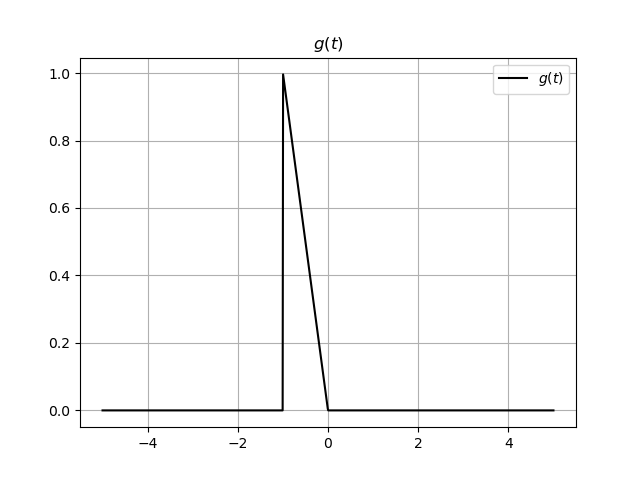
\includegraphics[width=\columnwidth]{graphs/g.png}

\end{flushleft}
\end{figure}
\end{column}
\begin{column}{0.5\textwidth}
\begin{figure}
\begin{flushleft}
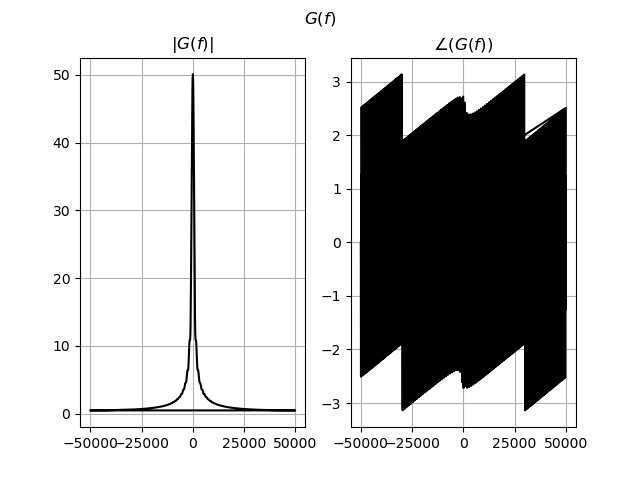
\includegraphics[width=\columnwidth]{graphs/fourier_g.png}

\end{flushleft}
\end{figure}
\end{column}
\end{columns}
\end{frame}



\begin{frame}{fragile}
\frametitle{$G_1(\omega)$}

\begin{flushleft}
Clearly, $g_1(t) = g(-t)$, and using \eqref{reverse}, we get:
\begin{align}
    G_1(f) = G(-f) = \frac{1}{4\pi^2f^2}(e^{-2\pi jf} + 2\pi jf e^{-2\pi jf} - 1)
\end{align}
\end{flushleft}
\end{frame}

\begin{frame}
  \frametitle{$g_1(t)$}
 \begin{columns}
\begin{column}{0.5\textwidth}
\begin{figure}
\begin{flushleft}
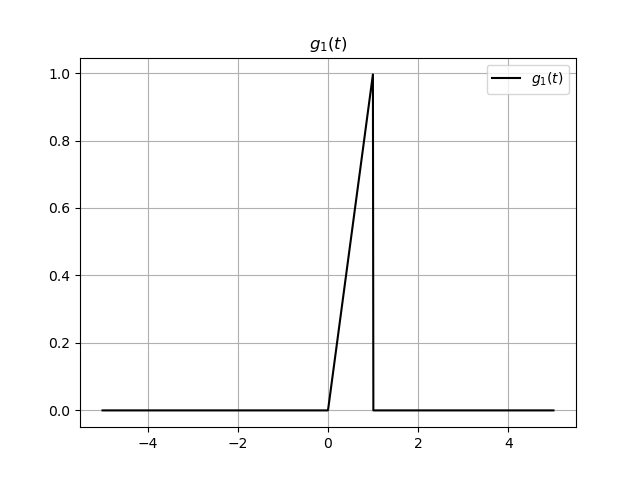
\includegraphics[width=\columnwidth]{graphs/g1.png}

\end{flushleft}
\end{figure}
\end{column}
\begin{column}{0.5\textwidth}
\begin{figure}
\begin{flushleft}
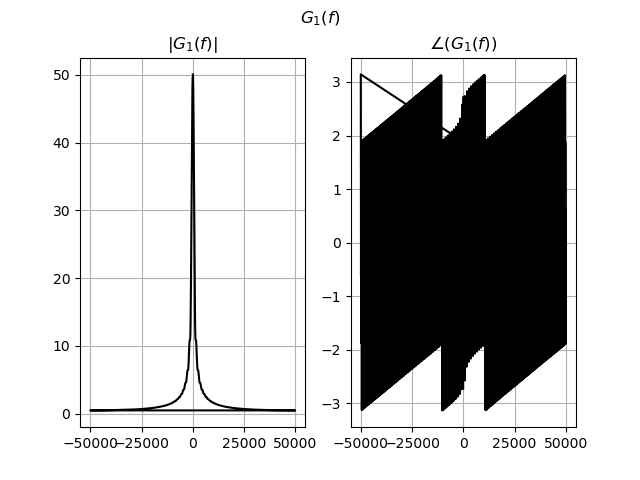
\includegraphics[width=\columnwidth]{graphs/fourier_g1.png}

\end{flushleft}
\end{figure}
\end{column}
\end{columns}
\end{frame}


\begin{frame}
    \frametitle{$G_2(\omega)$}
    \begin{flushleft}
    Also, $g_2(t) = g(-t-1)$. Thus, from \eqref{shift} and \eqref{reverse}, we get:

\begin{align}
   g(t-1) \fourier e^{-2\pi jf}G(f)\\
    g(-t-1) \fourier e^{2\pi jf} G(-f)\\
    g_2(t) \fourier e^{2\pi jf}G(-f) \\
   g_2(t) \fourier \frac{1}{4\pi^2f^2}(1 + 2\pi jf  - e^{2\pi jf})\\
   \implies G_2(\omega) =  \frac{1}{4\pi^2f^2}(1 + 2\pi jf  - e^{2\pi jf})
\end{align}
  \end{flushleft}
\end{frame}


\begin{frame}
  \frametitle{$g_2(t)$}
 \begin{columns}
\begin{column}{0.5\textwidth}
\begin{figure}
\begin{flushleft}
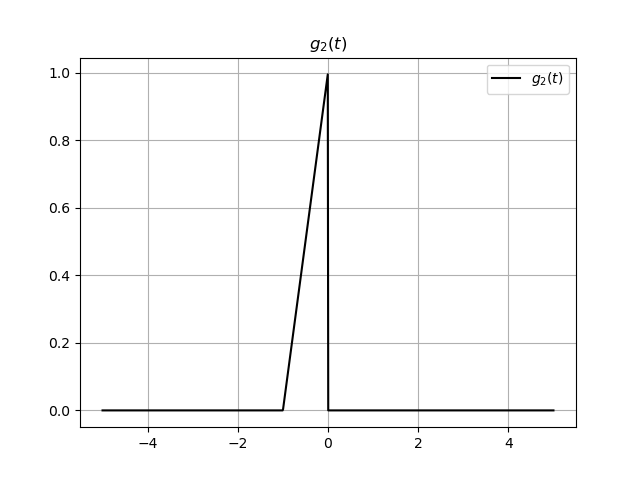
\includegraphics[width=\columnwidth]{graphs/g2.png}

\end{flushleft}
\end{figure}
\end{column}
\begin{column}{0.5\textwidth}
\begin{figure}
\begin{flushleft}
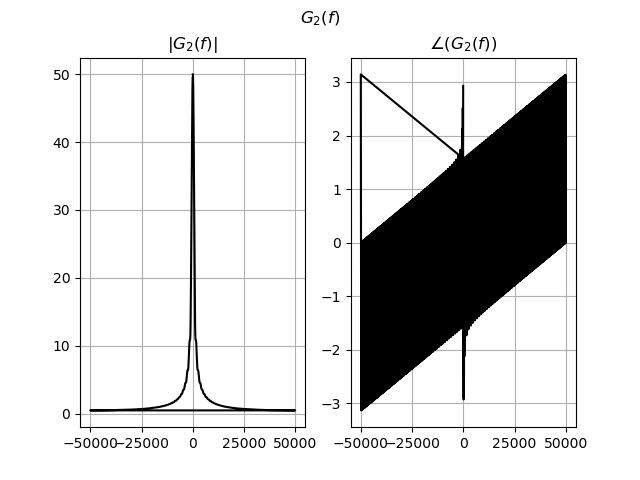
\includegraphics[width=\columnwidth]{graphs/fourier_g2.png}

\end{flushleft}
\end{figure}
\end{column}
\end{columns}
\end{frame}



\begin{frame}
    \frametitle{$G_3(\omega)$}
    \begin{flushleft}
Also, $g_3(t) = g\brak{t - \frac{1}{2}} + g\brak{-t - \frac{1}{2}}$. Thus, 
\begin{align}
    g_3(t) \fourier e^{-j\pi f}G(f) + e^{j\pi f}G(-f)\\
    G_3(f)= \frac{e^{-j\pi f}}{4\pi^2f^2}\sbrak{e^{2\pi jf} - 2\pi jfe^{2\pi jf} - 1} + \\
    \frac{e^{j\pi f}}{4\pi^2f^2}\sbrak{ e^{-2\pi jf} + 2\pi jfe^{-2\pi jf} -1}\\
        G_3(f) = \frac{j}{2\pi f}\sbrak{e^{-\pi jf} - e^{\pi jf}}=\frac{\sin{\pi f}}{\pi f} = sinc(f)
    \end{align}
    where $sinc(t)$, the sampling function is defined as:
\begin{align}
    sinc(t) = 
    \begin{cases}
    1 & t = 0\\
    \frac{\sin(\pi t)}{\pi t} & otherwise
    \end{cases}
\end{align}
    \end{flushleft}
\end{frame}

\begin{frame}
  \frametitle{$g_3(t)$}
 \begin{columns}
\begin{column}{0.5\textwidth}
\begin{figure}
\begin{flushleft}
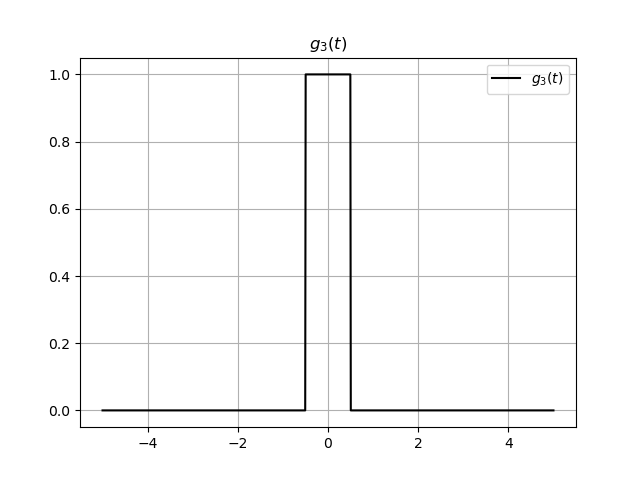
\includegraphics[width=\columnwidth]{graphs/g3.png}

\end{flushleft}
\end{figure}
\end{column}
\begin{column}{0.5\textwidth}
\begin{figure}
\begin{flushleft}
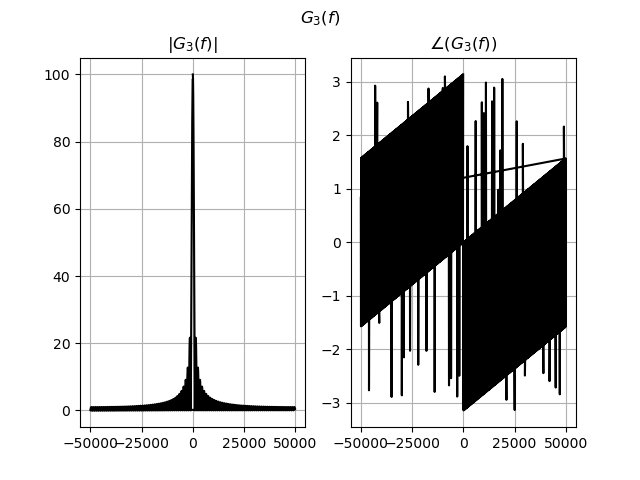
\includegraphics[width=\columnwidth]{graphs/fourier_g3.png}

\end{flushleft}
\end{figure}
\end{column}
\end{columns}
\end{frame}

\end{document}
